\documentclass[a4paper, 12pt]{article}
\usepackage[T2A]{fontenc}
\usepackage[utf8]{inputenc}
\usepackage[english,russian]{babel}
\usepackage{amsmath, amsfonts, amssymb, amsthm, mathtools, misccorr, indentfirst, multirow}
\usepackage{wrapfig}
\usepackage{graphicx}
\usepackage{subfig}
\usepackage{adjustbox}

\title{Лабораторная работа 4.7.1\\Двойное лучепреломление}
\author{Нехаев Александр, гр. 654}
\date{\today}
\begin{document}
	\maketitle
	\pagenumbering{gobble}
	\newpage
	\pagenumbering{arabic}
	\tableofcontents
	\newpage
	\section{Введение}
	\paragraph{Цель работы:}
	изучение зависимости показателя преломления необыкновенной волны от направления в двоякопреломляющем кристалле; определение главных показателей преломления $n_0$ — обыкновенной и $n_e$ — необыкновенной волны в кристалле; наблюдение эффекта полного внутреннего отражения.\par
		\paragraph{В работе используются:}
	гелий-неоновый лазер, вращающийся столик с неподвижным лимбом, призма из исландского шпата, поляроид.
	\section{Теоретические основы}
	\paragraph{Двойное лучепреломление.}
	При падении световой волны на границу изотропной среды ы этой среде от границы распространяется одна волна. Если среда анизотропна, то в ней в общем случае возникают две волны, распространяющиеся от границы в разных направлениях и с разными скоростями. Это явление называется \textit{двойным лучепреломлением}.
	\paragraph{Плоские волны в кристаллах.}
	В отсутствие электрических зарядов и токов уравнения Максвелла имеют вид
	\begin{equation}
		\mathrm{rot}\vec{H}=\frac{1}{c}\frac{\partial\vec{D}}{\partial t},\quad \mathrm{rot}\vec{E}=-\frac{1}{c}\frac{\partial\vec{B}}{\partial t}
		\label{eq:Maxwell}
	\end{equation}
	Если среды прозрачны и однородны, то в них могут распространяться плоские монохроматические волны. Запишем такую волну в комплексном виде:
	\begin{equation}
		\vec{E}=\vec{E_0}e^{i\left(\omega t-\vec{k}\vec{r}\right)};\quad \vec{B}=\vec{H}=\vec{H_0}e^{i\left(\omega t-\vec{k}\vec{r}\right)};\quad \vec{D}=\vec{D_0}e^{i\left(\omega t-\vec{k}\vec{r}\right)}
	\end{equation}
	Здесь $\omega$ — круговая частота, $\vec{k}$ — волновой вектор, а амплитуды $\vec{E_0}$, $\vec{H_0}$, $\vec{D_0}$ постоянны. Вектор $\vec{B}$ совпадает с $\vec{H}$, так как $\mu=1$. Обозначим координатные орты через $\vec{e_x},\vec{e_y},\vec{e_z}$ и получим:
	\begin{equation}
		\mathrm{rot}\vec{H}=\left|
		\begin{matrix}
			\vec{e_x} && \vec{e_y} && \vec{e_z}\\
			\frac{\partial}{\partial x} && \frac{\partial}{\partial y} && \frac{\partial}{\partial z}\\
			H_x && H_y && H_z
		\end{matrix}
		\right|=
		-i\left|
		\begin{matrix}
			\vec{e_x} && \vec{e_y} && \vec{e_z}\\
			k_x && k_y && k_z\\
			H_x && H_y && H_z
		\end{matrix}
		\right|=
		-i\left[\vec{k}\vec{H}\right]
	\end{equation}
	Аналогично для $\mathrm{rot}\vec{E}$. В результате (\ref{eq:Maxwell}) перейдут в 
	\begin{equation}
		\left[\vec{k}\vec{H}\right]=-\frac{\omega}{c}\vec{D};\quad\left[\vec{k}\vec{E}\right]=\frac{\omega}{c}\vec{B}
	\end{equation}\par
	Введем единичный вектор нормали $\vec{N}$ к фронту волны и скорость распространения фронта в направлении этой нормали $v$. Тогда $\vec{k}=\frac{\omega}{v}\vec{N}$ и предыдущие соотношения перейдут в
	\begin{equation}
		\vec{D}=-\frac{c}{v}\left[\vec{N}\vec{H}\right];\quad\vec{B}=\frac{c}{v}\left[\vec{N}\vec{E}\right].
		\label{eq:2}
	\end{equation}
	Отсюда видно, что векторы $\vec{D}$, $\vec{H}$, $\vec{H}$ взаимно перпендикулярны. Значит плоские волны в кристалле поперечны в отношении векторов $\vec{D}$ и $\vec{H}$. Однако в общем случае они не поперечны в отношении векторов $\vec{E}$.\par
	\begin{wrapfigure}{1}{4cm}
		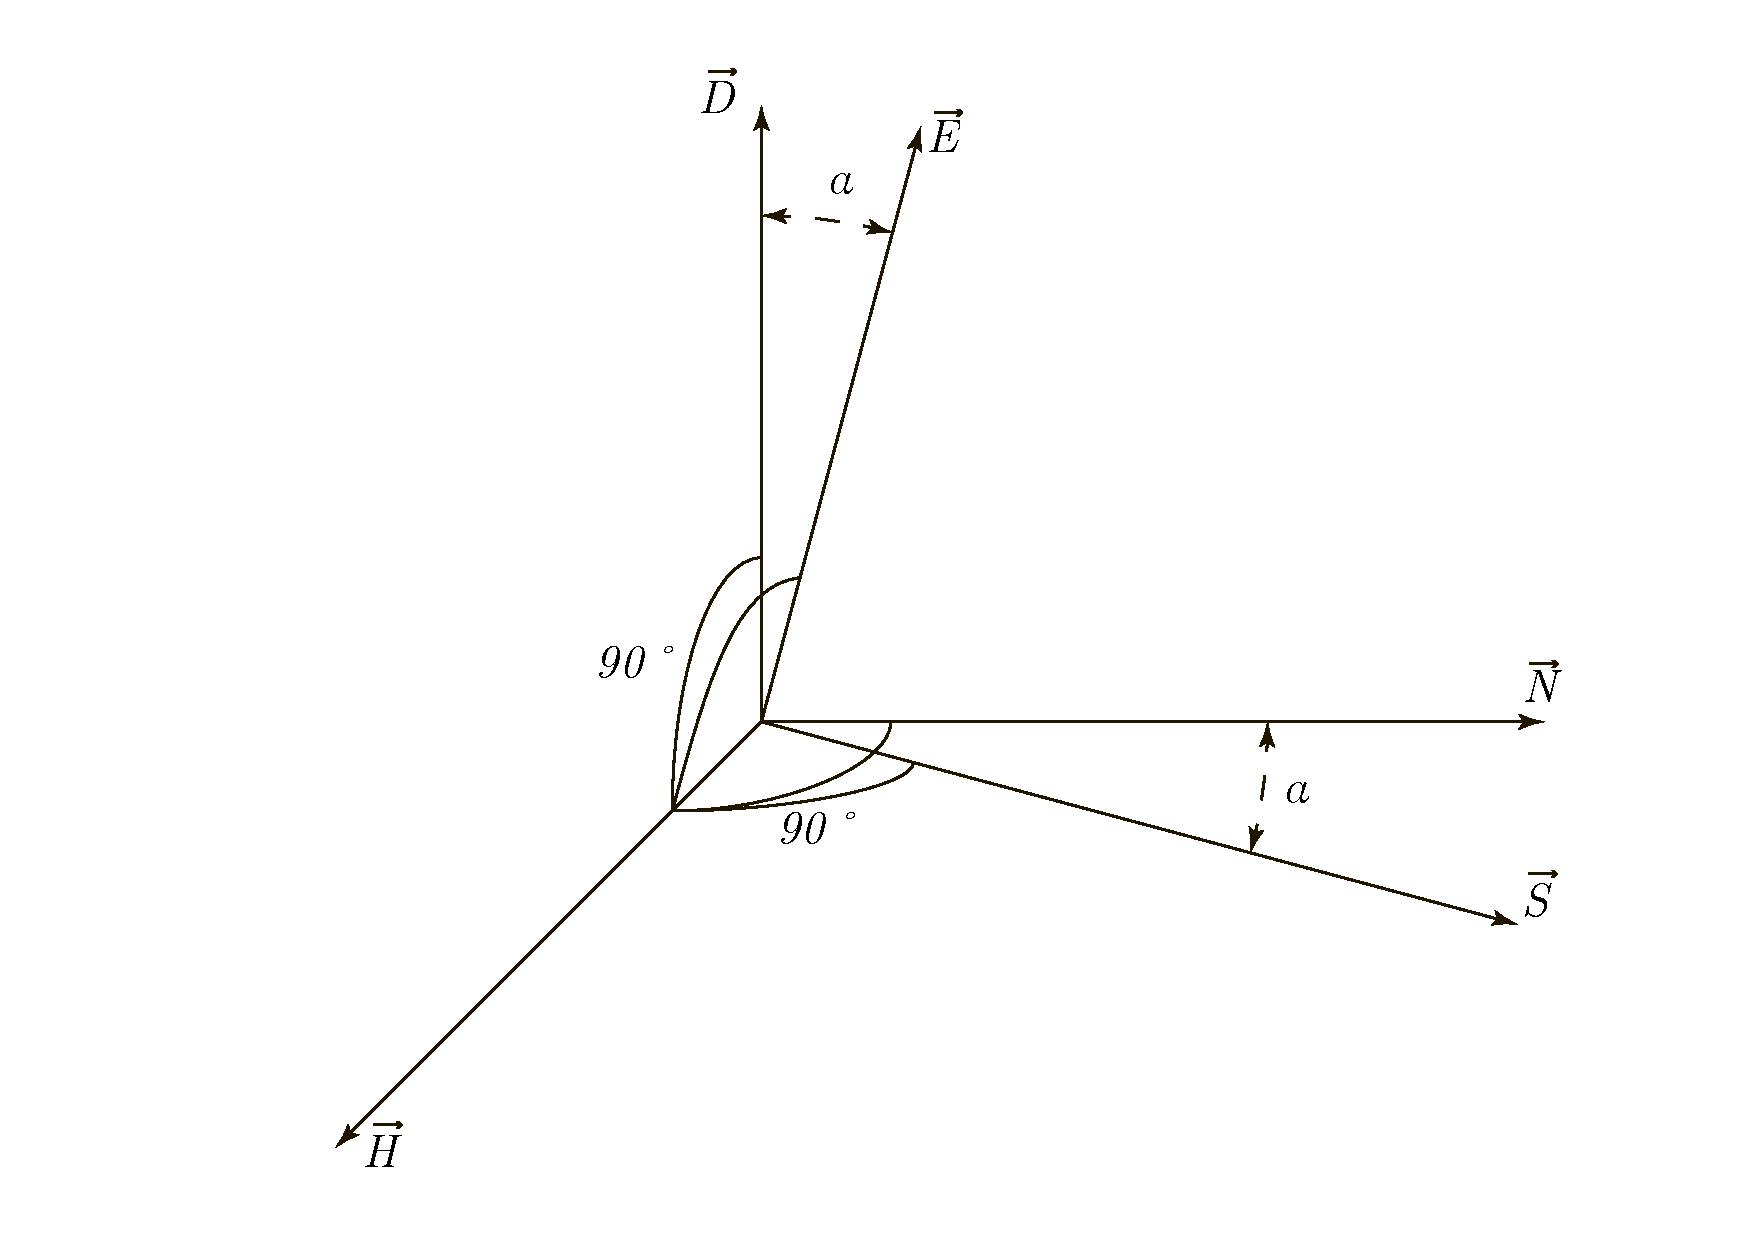
\includegraphics[scale=0.2]{DENS.pdf}
		\caption{Расположение векторов $\vec{D},\vec{E},\vec{N},\vec{S}$ в анизотропной среде}
		\label{fig:DENS}
	\end{wrapfigure}
	В изотропной среде: 
	\begin{equation}
		\vec{D}=\varepsilon\vec{E}
	\end{equation}
	$\varepsilon$ — диэлектрическая проницаемость\par
	В анизотропной среде:
	\begin{equation}
		D_i=\sum_{j}\varepsilon_{ij}\quad\left(i,j=x,y,z\right)
	\end{equation}
	Плоскость $\left(\vec{E},\vec{H}\right)$ обладает тем свойством, что перпендикуляр к ней определяет направление вектора Пойнтинга $\vec{S}=\frac{c}{4\pi}\left[\vec{E}\vec{H}\right]$, т.е. направление распространения световых волн. Четыре вектора $\vec{D},\vec{E},\vec{N},\vec{S}$ лежат в одной плоскости, перпендикулярной вектору $\vec{H}$. Взаимное расположение этих векторов показано на рис. \ref{fig:DENS}.
	\paragraph{Оптически одноосные кристаллы.}
	Всю совокупность возможных значений тензора диэлектрической проницаемости можно представить при помощи трехосного эллипса.\par
	$e_x,e_y,e_z$ — главные значения диэлектрической проницаемости\par
	$\sqrt{e_x},\sqrt{e_y},\sqrt{e_z}$ — главные показатели преломления.\par
	\begin{equation}
		D_x=\varepsilon_xE_x,\quad D_y=\varepsilon_yE_y,\quad D_z=\varepsilon_zE_z
	\end{equation}\par
	В оптически одноосном кристалле эллипсоид диэлектрической проницаемости представляет собой эллипсоид вращения. В нем оптическая ось совпадает совпадает с осью вращения эллипсоида диэлектрических проницаемостей. Для главных значений диэлектрической проницаемостей приняты обозначения: $\varepsilon_z=\varepsilon_\parallel$ и $\varepsilon_x=\varepsilon_y=\varepsilon_\perp$. Связь между проекциями векторов $\vec{D}$ и $\vec{E}$ на оптическую ось кристалла ($\vec{D}_\parallel$ и $\vec{E}_\parallel$) и на плоскость, перпендикулярную оси ($\vec{D}_\perp$ и $\vec{E}_\perp$):
	\begin{equation}
		\vec{D}_\parallel=\varepsilon_\parallel\vec{E}_\parallel,\quad \vec{D}_\perp=\varepsilon_\perp\vec{E}\perp.
		\label{eq:4}
	\end{equation}
	\par
	\begin{wrapfigure}{1}{7cm}
		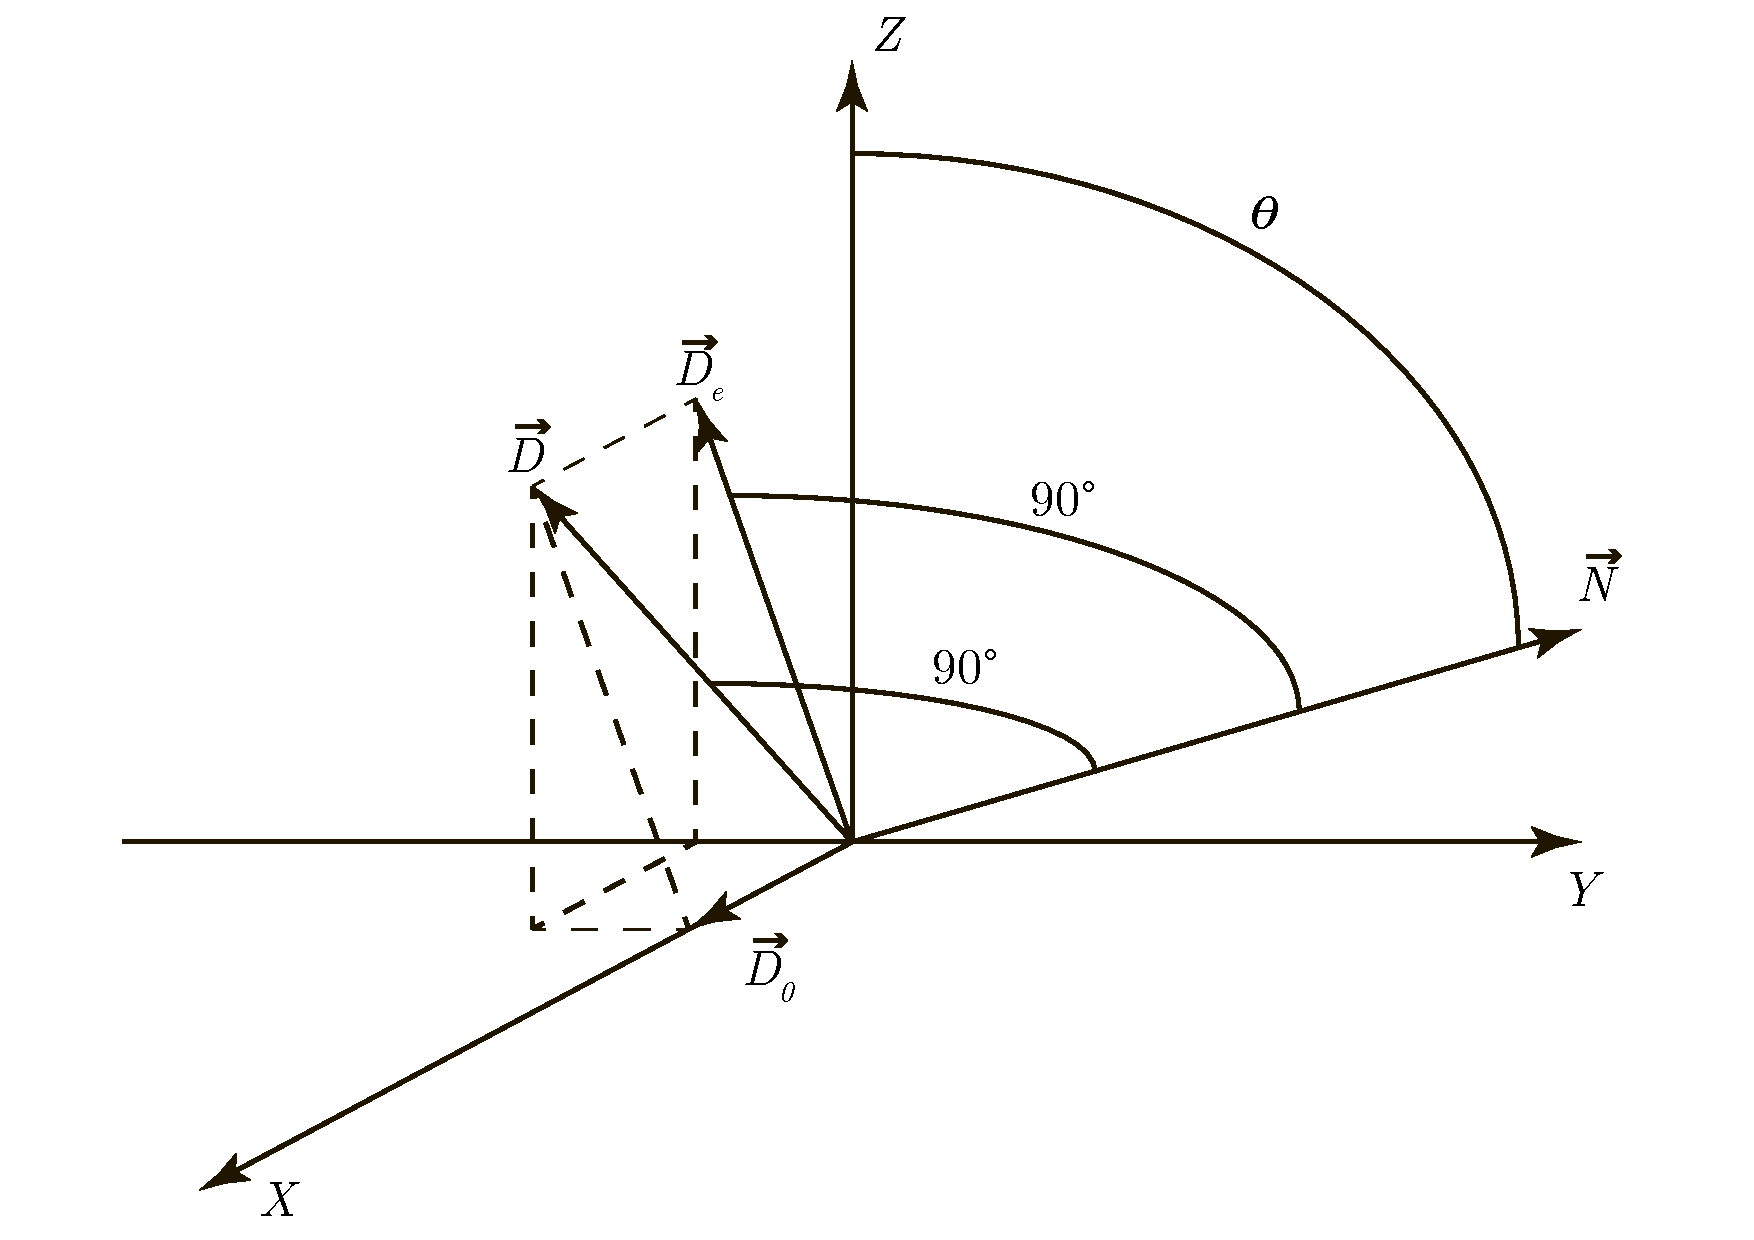
\includegraphics[scale=0.26]{ND_Location.pdf}
		\caption{Расположение векторов $\vec{N}$ и $\vec{D}$ в анизотропной среде: $\left(\vec{D}=\vec{D}_o+\vec{D}_e; \vec{D}_o\perp\vec{D}_e;\vec{D}\perp\vec{N}\right)$; $\vec{N}$ и $\vec{D}_e$ лежат в плоскости  $(Z,Y)$; $\vec{D}_o$ перпендикулярен плсокости $(Z,Y)$}
		\label{fig:ND_Location}
	\end{wrapfigure}
	Волну, распространяющуюся в одноосном кристалле, можно разделить на две линейно поляризованные волны: обыкновенную, вектор электрической индукции $\vec{D}_o$ которой перпендикулярен главному сечению, и необыкновенную, с вектором электрической индукции $\vec{D}_e$, лежащим в главном сечении (рис. \ref{fig:ND_Location}). \textit{Главным сечением кристалла} называется плоскость, в которой лежит оптическая ось кристалла и нормаль к фронту волны.\par
	Рассмотрим вначале обыкновенную волну, в которой вектор $\vec{D}_o$ перпендикулярен главному сечению. Тогда $D_{oz}=0$, и из условия $D_z=\varepsilon_zE_z$ следует, что $E_oz=0$.\par
	Кроме того, так как $D_oy=\varepsilon_\perp E_{oy}$ и $D_{ox}=\varepsilon_\perp E_{ox}$, то можно записать
	\begin{equation}
		\vec{D}_o=\varepsilon_\perp\vec{E}_o.
		\label{eq:5}
	\end{equation}
	\par
	Таким образом, для обыкновенной волны материальное уравнение имеет такой же вид, как и в изотропной среде. Найдем с помощью этого уравнения скорость распространения обыкновенной волны и соответствующий показатель преломления. Из (\ref{eq:2}) имеем
	\begin{equation}
		D_o=\frac{c}{v_o	}H_o,\quad H_o=\frac{c}{v_o}E_o
	\end{equation}
	или, учитывая (\ref{eq:5}),
	\begin{equation}
		\varepsilon_\perp E_o=\frac{c}{v_o}H_o,\quad H_o=\frac{c}{v_o}E_o,
	\end{equation}
	откуда
	\begin{equation}
		v_o=\frac{c}{\sqrt{\varepsilon_\perp}}\quad\text{и}\quad n_o=\frac{c}{v_o}=\sqrt{\varepsilon_\perp}.
	\end{equation}
	\par
	Таким образом, скорость распространения обыкновенной волны и её показатель преломления не зависят от направления распространения.\par
	У необыкновенной волны вектор $\vec{D}_e$ не параллелен $\vec{E}_e$, и связь между сложнее, чем в (\ref{eq:5}).\par
	Для того чтобы найти скорость распространения $v$ и показателя преломления необыкновенной волны $n=c/v$, достаточно найти связь между вектором электрической индукции этой волны $\vec{D}_e$ и проекцией на него вектора электрического поля волны $E_{eD}$. Тогда, подставляя $D_e=\varepsilon E_{eD}$ в (\ref{eq:2}), приходим к соотношениям
	\begin{equation}
		\varepsilon E_{eD}=\frac{c}{v}H_e;\quad H_e=\frac{c}{v}E_{eD},
	\end{equation}
	формально тождественным с соотношениями для обыкновенной волны. Роль величины $\varepsilon_\perp$ теперь играет величина $\varepsilon$, а показатель преломления необыкновенной волны равен $\sqrt{\varepsilon}$.\par
	Найдем связь между $D_e$ и $E_{eD}$. Для этого разложим векторы $\vec{D}_e$ и $\vec{E}_e$ на составляющие, параллельные и перпендикулярные оси кристалла:
	\begin{equation}
		\vec{D}_e=\vec{D}_{e\parallel}+\vec{D}_{e\perp}.
	\end{equation}
	\begin{equation}
		\vec{E}_e=\vec{E}_{e\parallel}+\vec{E}_{e\perp}.
	\end{equation}
	Учитывая (\ref{eq:4}), находим
	\begin{equation}
		E_{eD}=\frac{\vec{E}_e\vec{D}_e}{D_e}=\frac{E_{e\parallel}D_{e\parallel}+E_{e\perp}D_{e\perp}}{D_e}=\frac{D_{e\parallel}^2/\varepsilon_\parallel+D_{e\perp}^2/\varepsilon_\perp}{D_e}
	\end{equation}
	или
	\begin{equation}
		E_{eD}=D_e\left(\frac{\sin^2\theta}{\varepsilon_\parallel}+\frac{\cos^2\theta}{\varepsilon_\perp}\right)=\frac{D_e}{\varepsilon},
	\end{equation}
	где $\theta$ — угол между оптической осью $Z$ и волновой нормалью $N$ (рис. \ref{fig:ND_Location}):
	\begin{equation}
		\sin\theta=\frac{D_{e\parallel}}{D_e},\quad\cos\theta=\frac{D_{e\perp}}{D_e}.
	\end{equation}
	Таким образом, $\varepsilon$ и соответственно скорость распространения и показатель преломления необыкновенной волны зависят от угла между оптической осью кристалла и направлением распространения волны.\par
	Выпишем выражение для показателя преломления необыкновенной волны $n=\sqrt{\varepsilon}$ через главные показатели преломления $n_o$, $n_e$ и угол $\theta$:
	\begin{equation}
		\frac{1}{\left[n\left(\theta\right)\right]^2}=\frac{\sin^2\theta}{n_e^2}+\frac{\cos^2\theta}{n_o^2}.
		\label{eq:7}
	\end{equation}
	\par
	При $n_o-n_e\ll n_o$ и $n_e$  (для исландского шпата $n_o=1,655$, $n_e=1,485$ для $\lambda=0,63\text{ мкм}$ (\ref{eq:7}) можно упростить:
	\begin{equation}
		n\left(\theta\right)\approx n_e+\left(n_o-n_e\right)\cos^2\theta.
	\end{equation}
	\paragraph{Двойное лучепреломление в призме из исландского шпата.} Рассмотрим, как по преломлению лучей в кристаллической призме можно определить показатели преломления для обыкновенной и необыкновенной волны. В работе исследуется одна из двух призм, составляющих поляризатор (рис. \ref{fig:prismAndRaypath}).
	\begin{figure}[h]
	\centering
		\subfloat[]{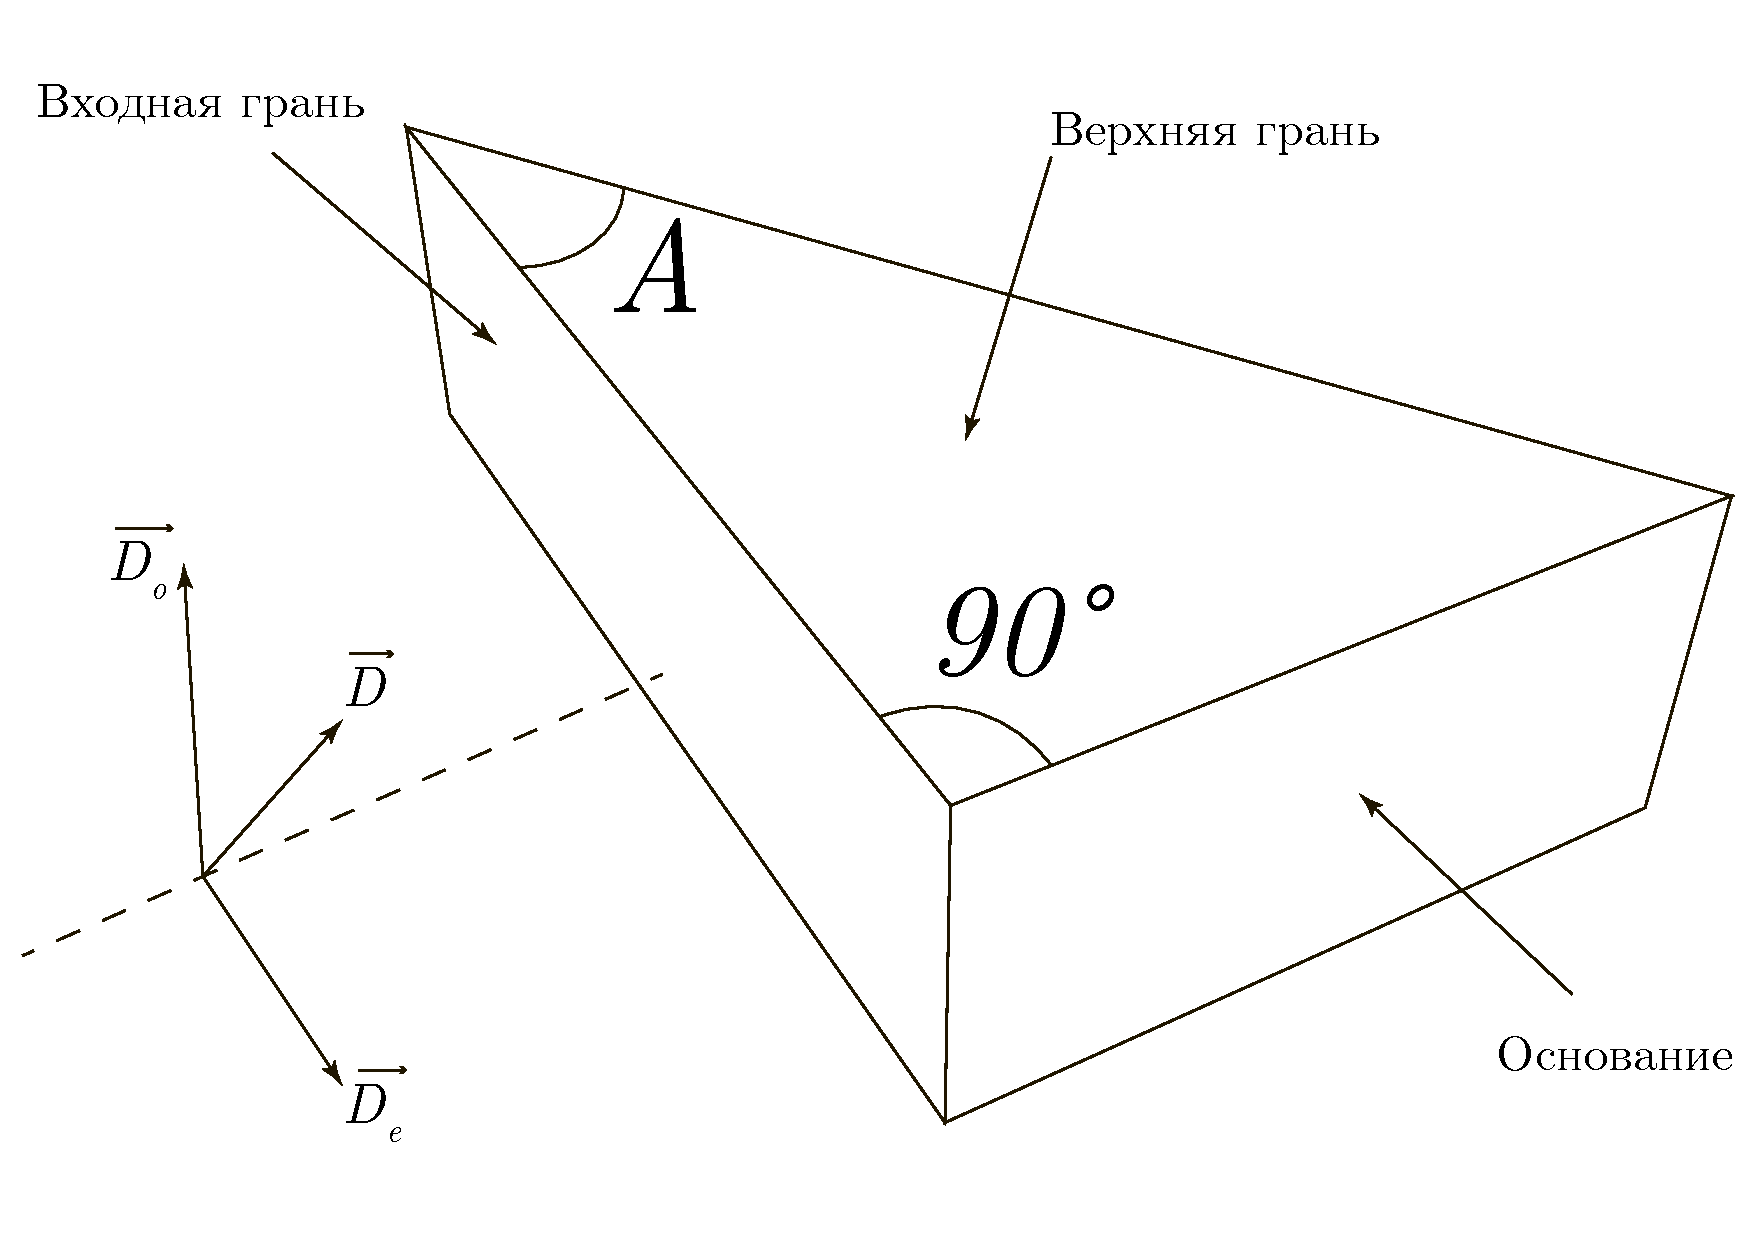
\includegraphics[scale=0.15]{Prism.pdf}}
		\quad
		\subfloat[]{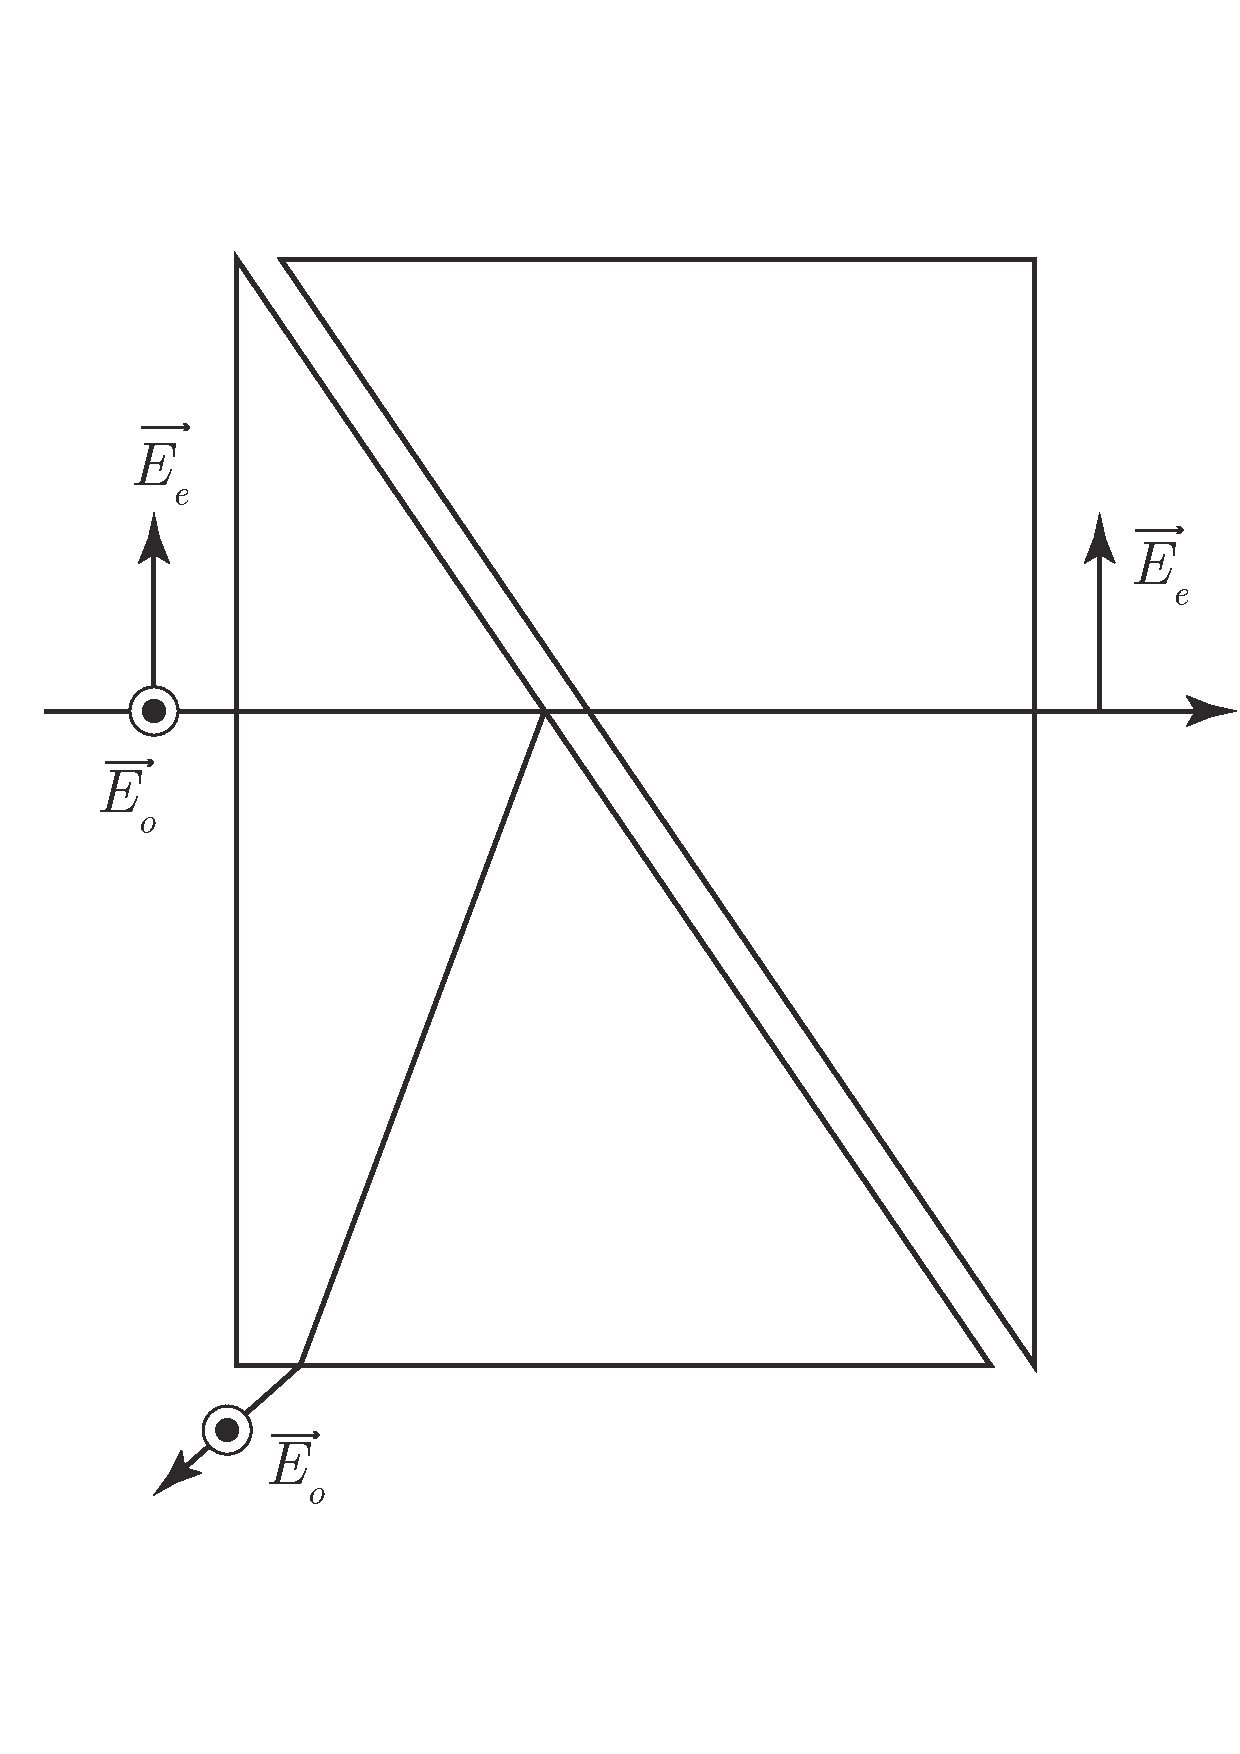
\includegraphics[scale=0.15]{Ray_Path.pdf}}
		\caption{(a) Исследуемая призма из исландского шпата. (b) Ход лучей в поляризационной призме.}
		\label{fig:prismAndRaypath}
	\end{figure}
	\par
	В исследуемой призме ось кристалла лежит в плоскости, параллельной верхней грани призмы, причем она параллельна входной грани призмы (длинному катету). При этом в обыкновенной волне вектор $\vec{D}_o$ перпендикулярен верхней грани призмы, а в необыкновенной волне вектор $\vec{D}_e$ параллелен верхней грани.\par
	\begin{wrapfigure}{1}{7cm}
		\centering
		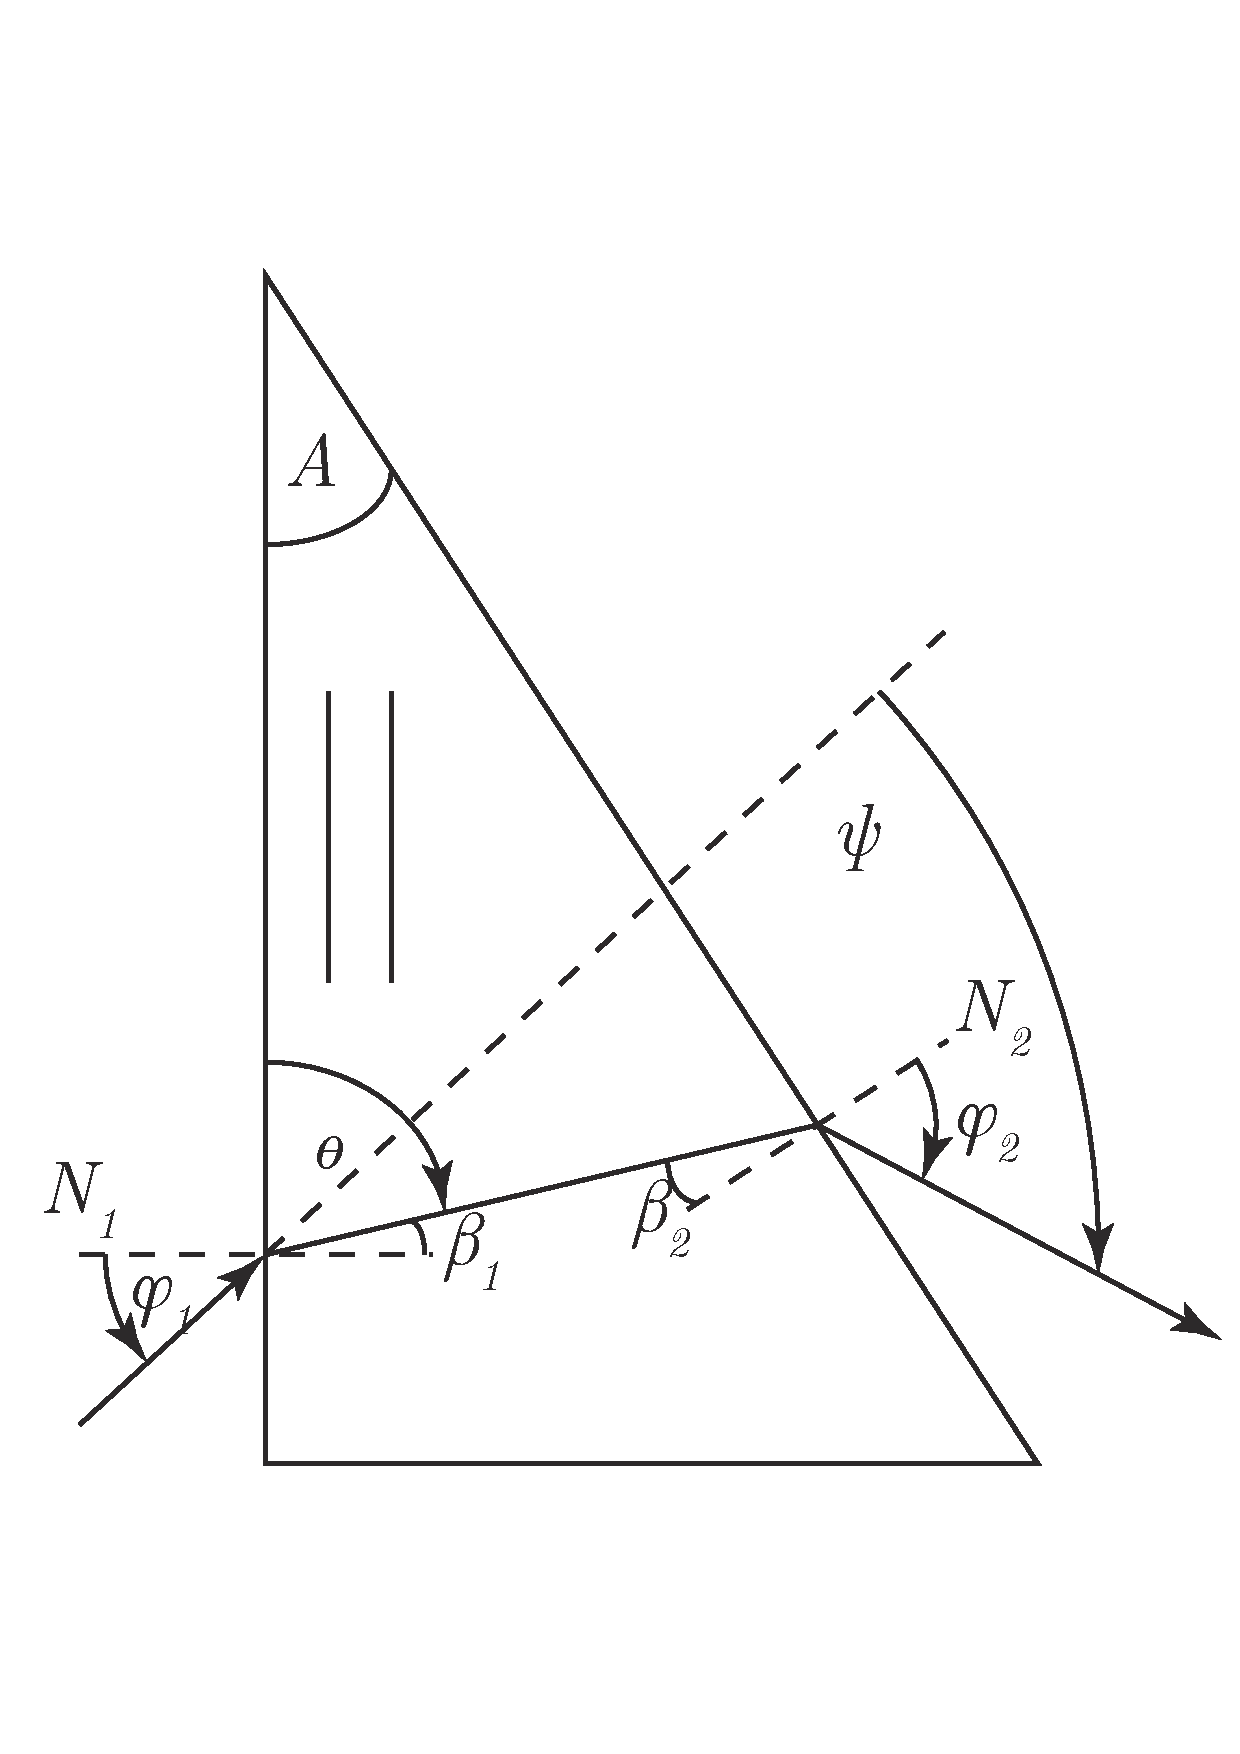
\includegraphics[scale=0.2]{Ray_Path_2.pdf}
		\caption{Ход лучей в призме}
		\label{fig:Ray_Path_2}
	\end{wrapfigure}
	Волну, падающую на входную грань призмы, можно представить в виде суммы двух волн ортогональных линейно поляризованных волн. Преломление этих двух волн на грани призмы можно рассматривать независимо. Волна, в которой вектор $\vec{D}$ направлен вертикально (перпендикулярно верхней грани и оси кристалла), внутри кристалла будет распространяться как обыкновенная. Для этой волны выполняется закон Снеллиуса, а показатель преломления призмы для нее равен $n_o=\sqrt{\varepsilon_\perp}$. Волна, в которой вектор $\vec{D}$ направлен горизонтально, в кристалле будет распространяться как необыкновенная. Для этой волны также будет выполняться закон Снеллиуса, но с тем отличием, что показатель преломления призмы для нее будет зависеть от угла между осью кристалла и волновой нормалью.\par
	 Значение показателя преломления и угол, под которым преломилась волна в призме, можно найти, измерив угол падения на входную грань призмы $\varphi_1$ и угол $\varphi_2$ на выходе призмы (рис. \ref{fig:Ray_Path_2}). Запишем закон Снеллиуса для одной из волн применительно к первой и второй граням призмы:
	 \begin{equation*}
	 	\sin\varphi_1=n\sin\beta_1;
	 \end{equation*}
	 \begin{equation*}
	 	\sin\varphi_2=n\sin\beta_2=n\sin\left(A-\beta_1\right).
	 \end{equation*}
	 При этом мы выразили угол падения на вторую грань призмы $\beta_2$ через угол преломления на первой грани призмы $\beta_1$ и угол при вершине призмы $A$. Как видно из рис. \ref{fig:Ray_Path_2}, эти углы связаны простым соотношением $A=\beta_1+\beta_2$. Учитывая, что угол преломления $\beta_1$ связан с углом $\theta$ между осью кристалла и волновой нормалью $\vec{N}$ соотношением $\theta+\beta_1=\pi/2$, находим $n$ и $\theta$:
	 \begin{equation}
	 	n=\frac{1}{\sin A}\sqrt{\sin^2\varphi_1+\sin^2\varphi_2+2\sin\varphi_1\sin\varphi_2\cos A};
	 	\label{eq:9}
	 \end{equation}
	 \begin{equation*}
	 \cos\varphi=\frac{\sin\varphi_1}{n}.	
	 \end{equation*}
	 Для обыкновенной волны $n$ не будет зависеть от угла $\theta$, а для необыкновенной волны зависимость $n$ от $\theta$ должна описываться выражением (\ref{eq:7}).\par
	 Показатель преломления призмы из изотропного материала удобно находить по углу наименьшего отклонения луча от первоначального направления. Угол отклонения луча призмой ($\psi$ на рис. \ref{fig:Ray_Path_2}) минимален для симметричного хода лучей, т.е. когда $\varphi_1=\varphi_2$. Тогда показатель преломления можно рассчитать по формуле
	 \begin{equation}
	 	n=\frac{\sin\left(\frac{\psi_m+A}{2}\right)}{\sin\left(\frac{A}{2}\right)},
	 	\label{eq:10}
	 \end{equation}
	 где $\psi_m$ — угол наименьшего отклонения.\par
	Если призма неизотропна, то этой формулой, строго говоря, можно воспользоваться только для обыкновенной волны, которая, как это было показано ранее, распространяется так же, как и в изотропной среде. Но если учесть, что угол при вершине призмы мал, и при угле наименьшего отклонения преломлённый луч в призме распространяется под углом к оси кристалла близким к $\pi/2$, то в качестве оценки формулу (\ref{eq:10}) можно использовать для определения $n_e$.
	\newpage
	\section{Экспериментальная установка}
	\begin{figure}[h]
		\centering
		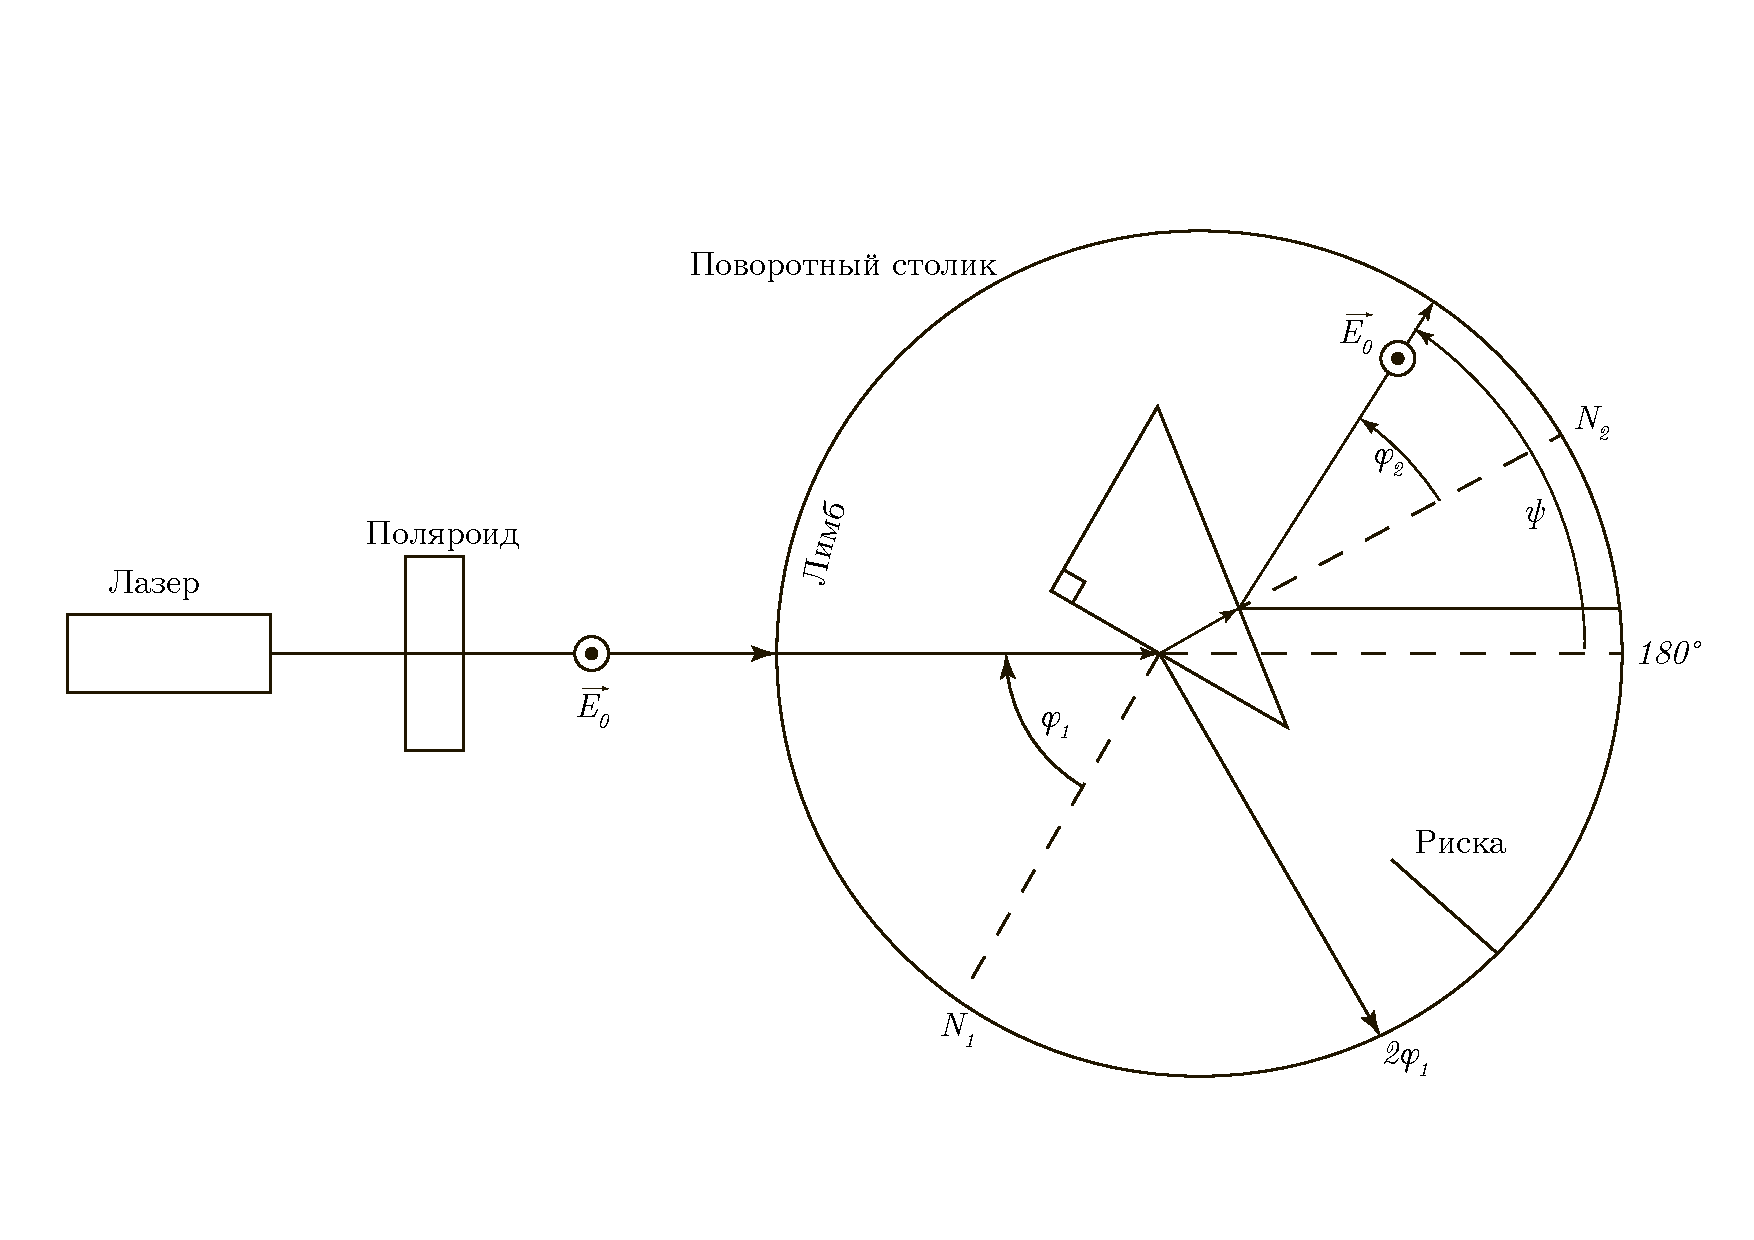
\includegraphics[scale=0.4]{ExperimentalScheme.pdf}
		\caption{Схема экспериментальной установки}
		\label{fig:mainScheme}
	\end{figure}
	Схема экспериментальной установки изображена на рис. \ref{fig:mainScheme}. Источником излучения служит He-Ne лазер ($\lambda=0.63$ мкм). Излучение лазера, поляризовано линейно за счет наличия брюстеровских окошек в кювете лазера. Направление вектора  $\vec{E}$ в луче можно изменять с помощью поляроида, установленного на выходе лазера. Исследуемая призма из исландского шпата закреплена в центре поворотного столика с неподвижным лимбом для отсчета углов.
	\section{Ход работы}
	\begin{enumerate}
		\item Определим угол $A$ при вершине призмы:
		\begin{equation*}
			\sin\frac{AC}{BC}=\frac{15}{23}\quad\angle A=\arcsin\frac{15}{23}=38^\circ
		\end{equation*}
		\item Определим разрешенное направление поляризатора: глядя через него на отраженный от горизонтальной поверхности стола дневной свет, установим его в положение минимального пропускания. Так как отраженный свет преимущественно поляризован так, что вектор $\vec{E}$ направлении параллельно отражающей поверхности, у настроенного на минимум пропускания поляризатора разрешенное направление $\vec{E}$ вертикально.
		\item Получим на лимбе изображения преломлённых лучей так, как показано, на рис. \ref{fig:mainScheme} (падающий и преломлённый лучи отклоняются от нормалей к преломляющим граням в сторону основания призмы). Установим поляризатор в луче лазера перед призмой. Вращая поляризатор, определи, какой луч соответствует вертикально поляризованному свету, а какой — горизонтально поляризованному; определим, какой из лучей представляет обыкновенную волну, а какой — необыкновенную.\par
		\begin{equation*}
			\text{Необыкновенная волна: }\vec{E} (\rightarrow),\quad\text{Обыкновенная волна: }\vec{E}(\uparrow)
		\end{equation*}
		\item Вращая столик с призмой, снимем зависимость углов отклонения на выходе из призмы для обыкновенной и необыкновенной волн от угла падения луча на призму; удобно определять координату $2\varphi_1$ луча, отраженного от входной грани призмы — длинного катет и координаты каждого из преломлённых лучей $(180^\circ+\psi)$ $(\text{или }180^\circ-\psi$.\par
		 Для проверки качества юстировки сначала проведите предварительную серию измерений, меняя угол падения $\varphi_1$ в диапазоне $10-70^\circ$ через $10^\circ$ ($2\varphi_1$ — через $20^\circ$ до $140^\circ$).\par
		 Для расчёта показателей преломления на компьютере с установленной программой SIGMA PLOT подготовим таблицу \ref{table:SIGMA_PLOT}.
		 \begin{table}
		 \centering
		 \begin{adjustbox}{angle=90}
		 	\centering
		 	\begin{tabular}{|c|c|c|c|c|c|c|c|c|c|c|c|c|c|c|}
		 	\hline
		 	№ & 1 & 2 & 3 & 4 & 5 & 6 & 7 & 8 & 9 & 10 & 11 & 12 & 13 & 14\\
		 	\hline
		 	$\varphi_1$ & 5 & 10 & 15 & 20 & 25 & 30 & 35 & 40 & 45 & 50 & 55 & 60 & 65 & 70\\
		 	\hline
		 	$\psi_0$ & 40 & 33 & 30 & 29	 & 28 & 27 & 27 & 28 & 29 & 30 & 31 & 32 & 35 & 37\\
		 	\hline
		 	$\psi_e$ & 25 & 29 & 31 & 21 & 20 & 21 & 21 & 22 & 23 & 24 & 25 & 27 & 30 & 32\\
		 	\hline
		 	$\varphi_{2o}$ & 73 & 61 & 53 & 47 & 41 & 35 & 30 & 26 & 22 & 18 & 14 & 10 & 8 & 5\\
		 	\hline
		 	$\varphi_{2e}$ & 58 & 51 & 44 & 39 & 33 & 29 & 24 & 20 & 16 & 12 & 8 & 5	 & 3 & 0\\
		 	\hline
		 	$\theta_o$ & 87 & 83,97 & 80,97 & 78,12 & 75,26 & 72,35 & 69,65 & 67,28 & 64,96 & 62,67 & 60,39 & 58,08 & 56,82 & 55,05\\
		 	\hline
		 	$\theta_o$ & 86,65	 & 83,33 & 	79,94 & 76,82 & 73,49 & 70,70 & 67,65 & 65,00 & 62,40 & 59,84 & 57,27 & 55,29 & 53,95 & 52,00\\
		 	\hline
		 	$\cos^2\theta_o$ & 0,00 & 0,01 & 0,02 & 0,04	 & 0,06 & 0,09 & 0,12 & 0,15 & 0,18 & 0,21 & 0,24 & 0,28 & 	0,30	 & 0,33\\
		 	\hline
		 	$\cos^2\theta_e$ & 0,00 & 0,01 & 0,03 & 0,05 & 0,08 & 0,11 & 0,14 & 0,18	 & 0,21 & 0,25 & 0,29 & 0,32	 & 0,35 & 0,38\\
		 	\hline
		 	$n_o$ & 1,667 & 1,652 & 1,649 & 1,661 & 1,661 & 1,649 & 1,649 & 1,664 & 1,671 & 1,669 & 1,658 & 1,638 & 1,656 & 1,640\\
		 	\hline
		 	$n_e$ & 1,492 & 1,495 & 1,482 & 1,499 & 1,478 & 1,512 & 1,508 & 1,521 & 1,526 & 1,525 & 1,515 & 1,521 & 1,540 & 1,526\\
		 	\hline
		 	\end{tabular}
		 \end{adjustbox}
		 \caption{Результат из SIGMA PLOT}
		 \label{table:SIGMA_PLOT}
		 \end{table}
		 \item Построим графики $n_o$ и $n_e\left(\theta\right)$ от $\cos^2\theta$ (см. рис. \ref{fig:graphic}) и определим главные показатели преломления $n_o$ и $n_e$. Сравним рассчитанные значения с табличными, приведенными в описании работы и оценим погрешность.
		 \begin{equation*}
		 	n_{o_0}=1.66\pm0.009\quad n_{e_0}=1.491\pm0.008
		 \end{equation*}
		 \item Из основной серии измерений определим средние значения углов наименьшего отклонения $\psi_m$; по формуле (\ref{eq:10}) рассчитаем показатели преломления $n_o$ и $n_e$.
		 \begin{equation*}
		 	n_o=-1.65 \quad n_e=-1.489
		 \end{equation*}
		 \newpage
		 \begin{figure}[h]
		 	\centering
		 	\includegraphics[scale=0.6]{Graphic.pdf}
		 	\caption{График, построенный в SIGMA PLOT}
		 	\label{fig:graphic}
		 \end{figure}
	\end{enumerate}
	\section{Вывод}
	Изучили зависимость показателя преломления необыкновенной волны от направления в двоякопреломляющем кристалле; определили главные показатели преломления.
\end{document}